% Deterministic and sparse autoencoders -- subsection of "Encoding",
% pulled in by sections/05-encoding.tex.

\subsection[Deterministic and sparse autoencoders]{Deterministic and Sparse Autoencoders}
\label{sec:ae}                           % \secref{sec:ae}

In addition to the VAEs described in \secref{sec:vae}, we trained two further variants at
both input resolutions ($128^3$ and $256^3$): a deterministic autoencoder, and a model with a
sparse convolutional encoder.

% ------------------------------------------------------------------------------
\subsubsection{Deterministic autoencoder}  % VAE with the variational part removed
\label{sec:ae_det}                       % \secref{sec:ae_det}

The deterministic autoencoder uses the same encoder and decoder as the VAE
(\secref{sec:vae_architecture}), with the variational part removed. Instead of two linear
layers predicting $\boldsymbol{\mu}$ and $\log\boldsymbol{\sigma}$, a single linear layer maps
the flattened encoder features directly to a latent code $\mathbf{z}$ of dimension
\TODO{100}. No sampling takes place, and the KL divergence term is dropped from the loss, so
the objective reduces to the weighted BCE, the clDice term and L2 weight regularization:
\begin{equation}
  \mathcal{L}_{\mathrm{AE}} = \mathcal{L}_{\mathrm{BCE\text{-}mod}}
  + \lambda\,(1 - \mathrm{clDice})
  + \mathcal{L}_{\mathrm{L2}}.
  \label{eq:ae_loss}                     % autoencoder loss without the KL term
\end{equation}
Without the KL term, the latent space is no longer pushed towards a unit Gaussian prior.
This means the model cannot be used to generate new trees by sampling, but the latent code
can still serve as a learned representation of each airway tree. Removing the KL term also
removes the trade-off between reconstruction quality and latent regularization. This lets us
test whether the KL term was responsible for the poor reconstructions of the VAE.

% ------------------------------------------------------------------------------
\subsubsection{Sparse encoder}           % encoder built on sparse voxel operators (XCube)
\label{sec:ae_sparse}                    % \secref{sec:ae_sparse}

\paragraph{Motivation.}                  % why sparsity suits airway trees
The second variant replaces the dense convolutional encoder with a sparse one, following
the sparse structure VAE of XCube \cite{ren2024}. Ren et al.\ argue that voxel grids are
flexible, can represent both bulky and thin structures, and allow fast querying and
processing. Sparse voxel representations go further by not storing any information for empty
regions, which makes them considerably more efficient \cite{ren2024}. This is particularly
relevant for airway trees: only a very small fraction of the $128^3$ or $256^3$ grid is
occupied, so a dense encoder spends most of its computation and memory on empty space.

\paragraph{Encoder design.}              % sparse conv + max pooling, as in XCube
As in XCube \cite{ren2024}, the encoder is built from neural network operators defined over
sparse voxel grids. It processes the input occupancy grid with a sparse convolutional neural
network that alternates between sparse convolutions and max pooling operations, reducing the
resolution step by step until it reaches the resolution of the latent representation. XCube
implements these operators on top of the VDB data structure \cite{museth2013}, whose compact
storage and fast look-up make sparse convolution and pooling efficient on the GPU. We
implemented the sparse encoder with \TODO{sparse convolution library, e.g.\ fVDB /
MinkowskiEngine / spconv}, using \TODO{number} sparse convolution layers and \TODO{number}
max pooling layers. The resulting sparse features are then \TODO{converted to a dense $7^3$
grid / globally pooled} and mapped to the latent code in the same way as in the dense model.

\paragraph{Decoder.}                     % decoder deliberately kept unchanged
We kept the decoder unchanged: it is the same dense decoder described in
\secref{sec:vae_architecture}. Note that XCube pairs its sparse encoder with a
structure-prediction decoder, which starts from the latent grid and progressively subdivides
existing voxels and prunes unnecessary ones until it reaches the output
resolution \cite{ren2024}. We did not adopt this decoder, so that any change in performance
could be attributed to the encoder alone. The sparse-encoder model was trained with the
\TODO{VAE objective of \secref{sec:vae_loss} / autoencoder objective of
Equation~\eqref{eq:ae_loss}}.

% ------------------------------------------------------------------------------
\subsubsection{Results}                  % same failure modes as the VAE
\label{sec:ae_results}                   % \secref{sec:ae_results}

Neither architecture produced satisfactory reconstructions. As with the VAE, reconstructions
of validation and test airway trees show \TODO{e.g.\ missing branches, broken connectivity,
blob-like structures} (Figure~\ref{fig:ae_recon}).

Both models also show the same overfitting behaviour as the VAE. The training loss decreases
steadily, while the validation loss does not follow it (Figure~\ref{fig:ae_curves}).
\TODO{Data augmentation and dropout were also applied to these models, without improvement.}

The deterministic autoencoder, the sparse-encoder model and the VAE all show the same
pattern. This suggests that the problem is not caused by the variational formulation or by
the type of encoder. More likely causes are the limited amount of training data relative to
model capacity and the difficulty of reconstructing thin, branching structures with a dense
voxel decoder.

\begin{figure}[htbp]                     % placeholder for AE and sparse reconstructions
  \centering                             % center the figure
  % 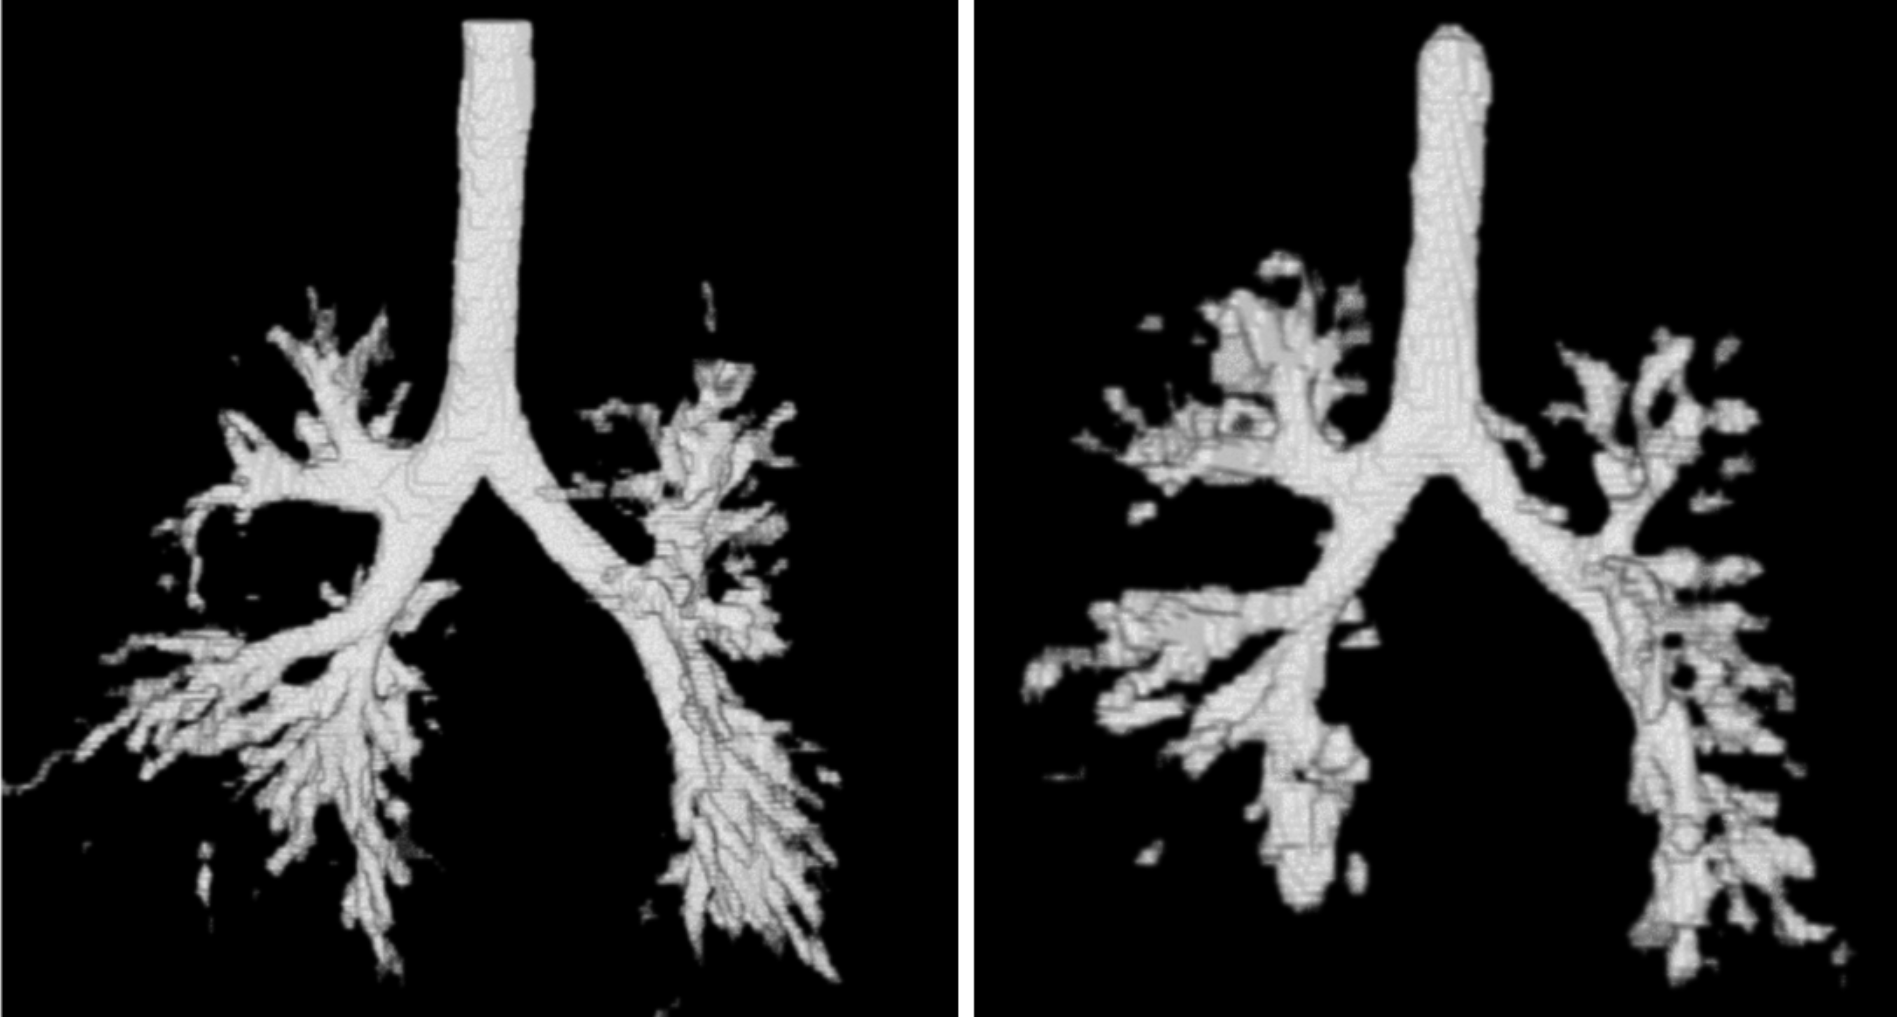
\includegraphics[width=\textwidth]{figures/ae_sparse_reconstructions.png}  % uncomment with your file
  \fbox{\parbox[c][4cm][c]{0.9\textwidth}{\centering [Reconstructions: autoencoder and sparse encoder]}}
  \caption{Original airway trees and their reconstructions from (a) the deterministic
           autoencoder and (b) the sparse-encoder model, for training and validation/test
           samples.}
  \label{fig:ae_recon}                   % referenced as Figure~\ref{fig:ae_recon}
\end{figure}

\begin{figure}[htbp]                     % placeholder for AE and sparse loss curves
  \centering                             % center the figure
  % \includegraphics[width=\textwidth]{figures/ae_sparse_curves.png}  % uncomment with your file
  \fbox{\parbox[c][4cm][c]{0.9\textwidth}{\centering [Loss curves: autoencoder and sparse encoder]}}
  \caption{Training and validation losses of (a) the deterministic autoencoder and (b) the
           sparse-encoder model. As with the VAE, the validation loss does not follow the
           training loss.}
  \label{fig:ae_curves}                  % referenced as Figure~\ref{fig:ae_curves}
\end{figure}
